\section{Architecture analysis}
\label{sec:architecture_analysis}

To understand better how the model was behaving and why it gave certain types of outputs rather than others, we used the python library Ecco\cite{alammar-2021-ecco}, which creates interactive visualizations that show at which layer of the architecture the final token has been decided, which input tokens contribute the most for a prediction, and many other insights on the model. \\
In particular, we used two different methods:
\begin{itemize}
    \item \textbf{Input Saliency}: used to show how much did each input token contribute to producing the output token
    \item \textbf{Neuron Activation Analysis}: used to examine underlying patterns in neuron activations using non-negative matrix factorization
\end{itemize}
\subsubsection*{Input Saliency}
To get a better grasp of the most useful information of the prompt, and to understand how we could modify it to achieve better results, we used the Gradient * input\cite{shrikumar2017learning} method. This technique calculates the partial derivatives of the output of the model and multiplies them with the input itself. Then the inputs with the highest scores are considered the ones that influenced the most the generation of the new tokens
\begin{equation*}
    score = x_i \bigtriangledown f(x_i)
\end{equation*}
where $f$ is the architecture output. \\
The main problem with the Gradient * input method is that only one input is considered. Integrated Gradients\cite{sundararajan2017axiomatic} solve this issue, computing the average gradient while the input varies along a linear path.
\begin{equation*}
    score = (x_i - x_i')\int_{\alpha = 0}^{1} \bigtriangledown f(x' + \alpha(x - x')) \,d\alpha 
\end{equation*}
Nevertheless, we used the Gradient * input method for computational issues ( The Integrated Gradients took too much RAM of the GPUs ).\\
In the images under, we underline some of the considerations we have done while defining the prompts.

\begin{figure*}[h!] 
    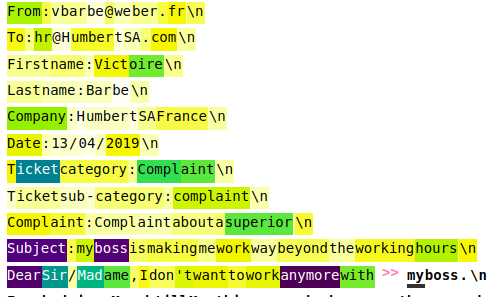
\includegraphics[width=0.6\textwidth]{images/Screenshot from 2022-11-26 17-19-27}
    \caption{Input Saliency: First token}
    \medskip
    \footnotesize
    To create the first token, the model focus on the elements that resemble the content of an email, in particular on the fact that it is indeed a 'Ticket'
    \label{fig:first_token}
\end{figure*}    

\begin{figure*}[h!] 
    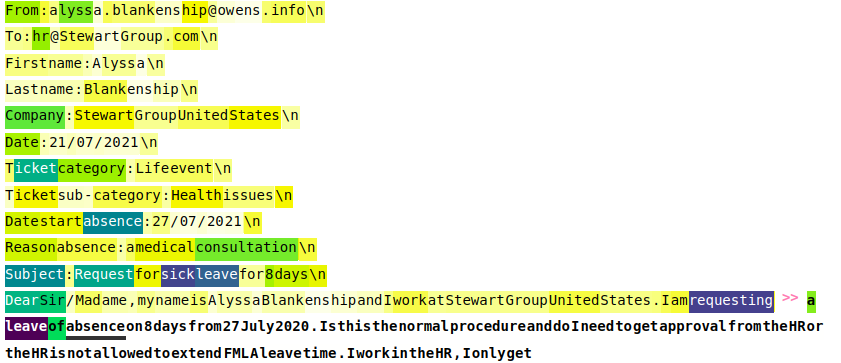
\includegraphics[width=0.8\textwidth]{images/Screenshot from 2022-11-26 18-18-28}
    \caption{Input Saliency: Subject}
    \medskip
    \footnotesize	
    Clearly stating the subject of the ticket helps the model create tokens that are on the right topic ( In this example 'days of absence')
    \label{fig:topic}
\end{figure*}    

\begin{figure*}[h!] 
    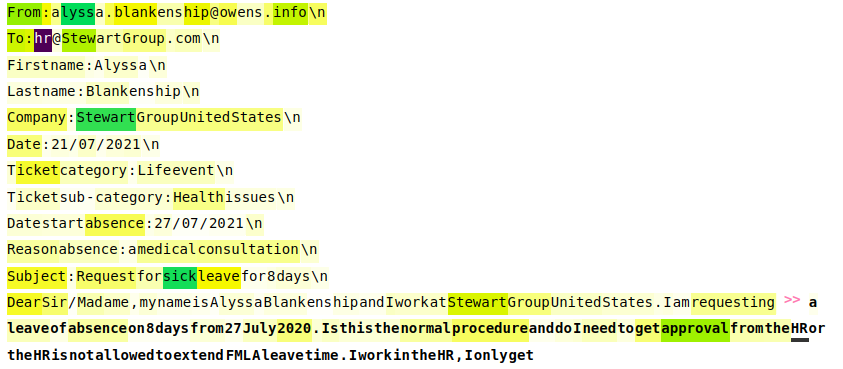
\includegraphics[width=0.85\textwidth]{images/Screenshot from 2022-11-26 18-18-40.png}
    \caption{Input Saliency: HR}
    \medskip
    \footnotesize
    Clearly stating that we are writing to hr can help the model know the context, and consecutively use a certain language, specific words\dots
    \label{fig:hr}
\end{figure*}    


\subsubsection*{Neuron Activation Analysis}
The Feed Forward Neural Network layer is one of the major components inside a transformer's block. To better understand how the neurons of different layers were 'activated' and how the neurons contributed towards each generated token, we exploited the Factor Analysis provided by Ecco. \\
Firstly, Ecco calculates the activation scores of each neuron over all layers, and then uses Non-negative Matrix Factorization (\autoref{fig:nmf}) to do dimensionality reduction on the matrix of activations, which will be reduced to a matrix $M{\times}T$, where $M$ is a parameter we decide and $T$ is the number of tokens, starting from a matrix $ ( n \cdot N ){\times}T$, where $n$ is the number of neurons per layer and $N$ is the number of layers. In GPT-J  $n = 16384$ and $N = 28$. \\
\begin{figure*}[h] 
    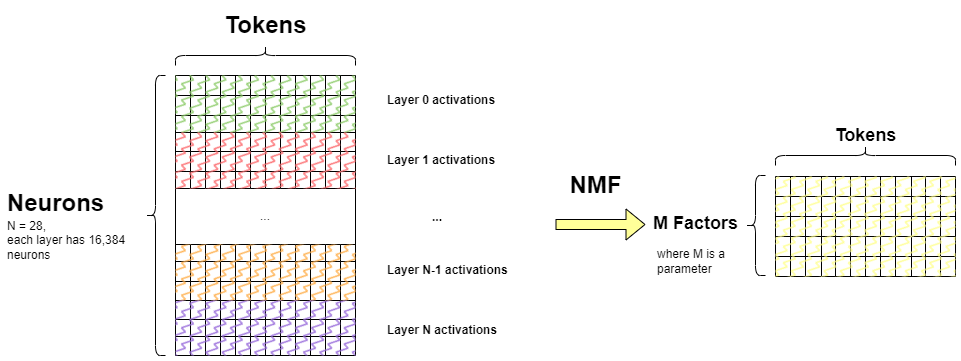
\includegraphics[width=\textwidth]{images/nmf.drawio}
    \caption{Non-negative Matrix Factorization on Activation Matrix}
    \label{fig:nmf}
\end{figure*}
Then, for each factor, which are the dimensionality-reduced layers, we visualize their activated neurons.
From the example in the \autoref{fig:Neuron_Activation_Analysis}, we can show for each factor what their main contributions are:
\begin{enumerate}
    \item Punctuation
    \item Mail prompt ( From, To, First Name, Last Name, Company\dots)
    \item New lines
    \item Dates
    \item First token, common across various GPT factors
    \item Medical terms ( usually terms related to the tickets' topic )
    \item People's names and contacts
    \item Company's name and contacts
    \item Ticket's subject ( Category, Sub-category and additional info )
    \item Email presentation ( 'Dear Sir/Madame\dots' )
\end{enumerate}

\begin{figure*}[h] 
    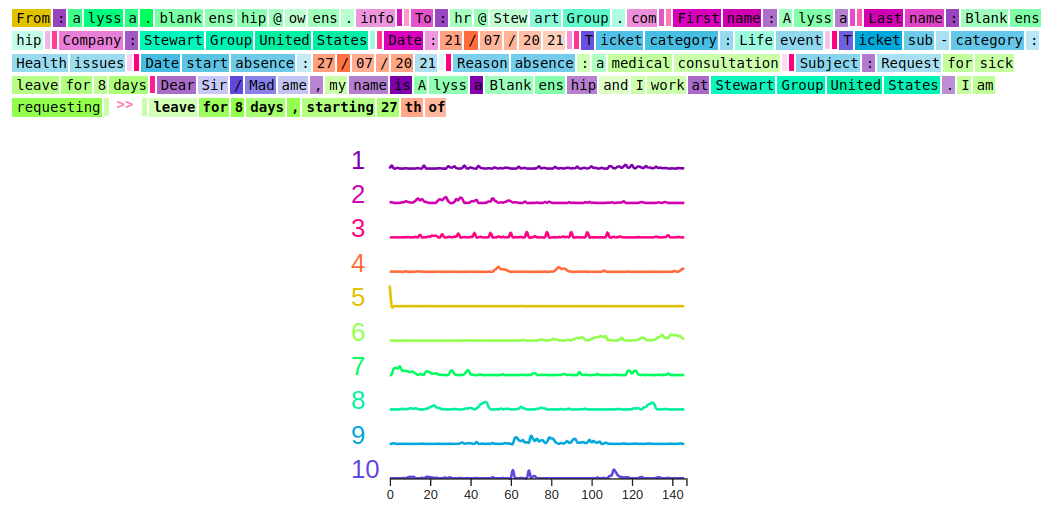
\includegraphics[width=\textwidth]{images/Screenshot from 2022-11-28 15-26-01.png}
    \caption{Neuron Activation Analysis}
    \label{fig:Neuron_Activation_Analysis}
\end{figure*}    


